\documentclass[12pt,oneside,final]{book}

\usepackage[portuges,brazil]{babel}
\usepackage[latin1]{inputenc}

\usepackage{indentfirst}
\usepackage{ae}
\usepackage{harvard}
\usepackage{amssymb,fancyhdr,fancybox,epsfig,psfrag,amsmath,tabularx}
\usepackage[paperwidth=8.5in,paperheight=11in,hmargin={25mm,20mm},vmargin={20mm,20mm}]{geometry} %tamanho letter
\usepackage{changepage}
\usepackage[table,xcdraw]{xcolor}
\usepackage{graphicx}
\usepackage{float}
\graphicspath{ {images/} }

\renewcommand*{\harvardand}{e}

\usepackage[color]{showkeys}
\definecolor{refkey}{rgb}{0.39,0.58,1}
\definecolor{labeled}{rgb}{1,0,0}
\usepackage[Lenny]{fncychap}
\setlength{\headheight}{15pt}

%=========================================== Headers =========================================
\renewcommand{\chaptermark}[1]{\markboth{\chaptername\ \thechapter. \ #1}{ }}
\renewcommand{\sectionmark}[1]{\markright{\thesection. \ #1}}
\fancyhead{}
\fancyfoot{}
\fancyhead[LO]{\nouppercase{\leftmark}}
\fancyhead[RO]{\thepage}

% Espacos H2, Hoo, L2, Loo
\newcommand\Hi{{\mathcal{H}}_{\infty}}
\newcommand\Hd{{\mathcal{H}}_{2}}
\newcommand\Li{{\mathcal{L}}_{\infty}}
\newcommand\Ld{{\mathcal{L}}_{2}}


\def\reais{{\rm I\kern-.17em R}} % R de reais
\def\Dest{{\rm I\kern-.17em D}} % R de reais
\newcommand{\Dgest}{\ensuremath{\mathcal{D}}}
\newcommand{\naturais}{\mathbb{N}}
\newcommand{\inteiros}{\mathbb{Z}_{+}}
\newcommand{\matlab}{{\sc Matlab}}

%super parenteses
\makeatletter
\def\Biggg#1{{\hbox{$\left#1\vbox to29\p@{}\right.\n@space$}}}
\newdimen\bracketwidth
\settowidth{\bracketwidth}{\Biggg(} \makeatother


%\newcommand{\carinha}{\raisebox{-.2ex}{\epsfxsize 3mm \epsffile{cara.eps}}}

% Bolds
\newcommand{\I}{{\bf I}}
\newcommand{\Z}{{\bf 0}}
\newcommand{\Bfres}{\mathcal{B}}

% funcoes
\newcommand{\Tr}{\mbox{Tr}}

% Referencia com parenteses
\newcommand{\bref}[1]{\mbox{(\ref{#1})}}

% Ambiente de equacoes
\newcommand\be{\begin{equation}}
\newcommand\ee{\end{equation}}
\newcommand\vi{\vspace{\baselineskip}}

% newtheorems e similares

\newtheorem{teorema}{\noindent{\bf Teorema} }[chapter]
\newtheorem{lema}{\noindent{\bf Lema} }[chapter]
\newtheorem{corolario}{\noindent{\bf Corol�rio} }[chapter]
\newenvironment{prova}{\noindent{\bf Prova:}}{\null\hfill $\rule{1.5mm}{1.5mm}$}
\newtheorem{definicao}{\noindent{\bf Defini��o} }[chapter]

\newcommand{\simplex}{\Delta_N}



\newcommand{\Aal}{A(\alpha)}
\newcommand{\Bal}{B(\alpha)}
\newcommand{\Cal}{C(\alpha)}
\newcommand{\Dal}{D(\alpha)}


\newcommand{\Pal}{P(\alpha)}
\newcommand{\Gal}{G(\alpha)}
\newcommand{\Hal}{H(\alpha)}
\newcommand{\Qal}{Q(\alpha)}
\newcommand{\Xal}{X(\alpha)}
\newcommand{\Xual}{X_1(\alpha)}
\newcommand{\Xdal}{X_2(\alpha)}

\newcommand{\Sfr}{\mathcal{S}}

\newcommand{\Xfal}{\mathcal{X}(\alpha)}
\newcommand{\Bfal}{\mathcal{B}(\alpha)}
\newcommand{\Qfal}{\mathcal{Q}(\alpha)}
\newcommand{\Sfal}{\mathcal{S}(\alpha)}

\newcommand{\Kfr}{\mathcal{K}}
\newcommand{\Ifr}{\mathcal{I}}
\newcommand{\Afr}{\mathcal{A}}
\newcommand{\Pfr}{\mathcal{P}}
\newcommand{\Cfr}{\mathcal{C}}
\newcommand{\Gfr}{\mathcal{G}}


\begin{document}

\pagenumbering{roman}
\pagestyle{plain}

%Tese em portugu�s
%================================================================================================
%================================= PRIMEIRA FOLHA INTERNA  ======================================
%================================================================================================
\vspace*{2.0cm}
\begin{center}
\large Ana Paula Cortina de Liz
\end{center}


\vspace*{6.8cm}

\begin{center}
{\sc \Large  Jogos digitais no processo de aprendizagem da l�ngua portuguesa como segunda l�ngua para alunos surdos. }
\end{center}

\vspace*{3.25cm}


\null \vfill

\begin{center}
Campinas\\2016
\end{center}
\newpage

%================================================================================================
%====================================== FOLHA DE ROSTO ==========================================
%================================================================================================

\begin{center}
\large Universidade Estadual de Campinas\\
Faculdade de Educa��o
\end{center}

\vspace*{1.5cm}
\begin{center}
\large Ana Paula Cortina de Liz
\end{center}


\vspace*{2.3cm}

\begin{center}
{\sc  Jogos digitais no processo de aprendizagem da l�ngua portuguesa como segunda l�ngua para alunos surdos.}
\end{center}

\vspace*{3.0cm}

\begin{flushright}
\begin{minipage}{9.0cm}
Trabalho de conclus�o de Curso apresentada � Faculdade Edu��o como parte dos
requisitos exigidos para a obten��o do Diploma de Gradua��o.

\vspace*{0.5cm}
Orientadora: Lilian Cristine Ribeiro Nascimento

\end{minipage}
\end{flushright}

\null \vfill
\begin{minipage}{7cm}
\small
Este exemplar corresponde � vers�o final do trabalho de conclus�o de curso defendida pela aluna,
e orientada pela Prof. Lilian Cristine Ribeiro Nascimento\\[4mm]
\rule{7.0cm}{0.2mm} \hfill 
\end{minipage}

\vspace*{0.5cm}

\begin{center}
Campinas\\2016
\end{center}

%================================================================================================
%============================== Ficha (Somente na vers�o final) =================================
%================================================================================================
\newpage

\begin{center}
\vspace*{10cm}
Remover p�gina?
Insira nesta p�gina a sua ficha catalogr�fica (somente vers�o final). Obs. � conveniente
converter o documento fornecido pela BAE (normalmente .doc) em um arquivo .ps. Para a vers�o
preliminar da tese (antes da defesa), simplesmente remova essa p�gina.
\end{center}
% Observa��o: a ficha fornecida pela BAE normalmente � fornecida em formato .doc. Existem diversas
% maneiras de converter .doc em .ps. 

% Descomente as duas pr�ximas linhas (e comente acima desde o begin{center} at� o end{center}) para inserir a ficha catalogr�fica caso a mesma j�  tenha sido convertida para .ps (no caso ficha.ps)

%\epsfxsize=0.925\columnwidth
%\epsffile{ficha.ps}

\null \vfill
\newpage

%================================================================================================
%============================== Folha de aprova��o (Somente na vers�o final) ====================
%================================================================================================


\begin{center}
\vspace*{10cm}
Remover p�gina?
Insira nesta p�gina a folha de aprova��o fornecida pelo seu programa de p�s-gradua��o (somente vers�o final). 
Obs. � conveniente scanear o documento e convert�-lo para o formato .ps. Para a vers�o
preliminar da tese (antes da defesa), simplesmente remova essa p�gina.
\end{center}

% Escanear a folha de aprova��o fornecida pela CPG e converter para .ps ou .eps. A id�ia
% � inserir como uma figura. � muito prov�vel que ser� necess�rio fazer ajustes no
% tamanho, mexendo no comando \epsfxsize

% Descomente as duas pr�ximas linhas (e comente acima desde o \begin{center} at� o \end{center})
%\epsfxsize=0.985\columnwidth
%\hspace*{-1.25cm}\epsffile{aprov.eps}

\null \vfill
\newpage
%Tese em portugu�s e ingl�s
%%================================================================================================
%================================= PRIMEIRA FOLHA INTERNA  ======================================
%================================================================================================
\vspace*{2.0cm}
\begin{center}
\large Fulano de Tal
\end{center}


\vspace*{4.8cm}

\begin{center}
{\sc \Large  Coloque aqui o t�tulo da tese; Coloque aqui o t�tulo \\ da tese;
Coloque aqui o t�tulo da tese;  Coloque aqui }
\end{center}

\vspace*{1cm}
\begin{center}
{\sc \Large  Place here the thesis' title;Place here the thesis'\\ title; Place here the thesis' title ;
Place here }
\end{center}

\vspace*{3.25cm}


\null \vfill

\begin{center}
Campinas\\2012
\end{center}
\newpage

%================================================================================================
%====================================== FOLHA DE ROSTO ==========================================
%================================================================================================

\begin{center}
\large Universidade Estadual de Campinas\\
Faculdade de Engenharia El�trica e de Computa��o
\end{center}

\vspace*{1.0cm}
\begin{center}
\large Fulano de Tal
\end{center}


\vspace*{1.3cm}

\begin{center}
{\sc  Coloque aqui o t�tulo da tese; Coloque aqui o t�tulo da tese;  \\ 
Coloque aqui o t�tulo da tese;  Coloque aqui o t�tulo da tese;}
\end{center}

\vspace*{0.5cm}

\begin{center}
{\sc   Place here the thesis' title;Place here the thesis'\\ title; Place here the thesis' title ;
Place here }
\end{center}

\vspace*{1.0cm}

\begin{flushright}
\begin{minipage}{11.0cm}
Tese de doutorado apresentada � Faculdade de Engenharia El�trica e de Computa��o como  parte dos
requisitos exigidos para a obten��o do t�tulo de Doutor em Engenharia El�trica. �rea de
concentra��o: Automa��o. 

\vspace*{0.5cm}

Doctorate thesis presented to the School of Electrical and Computer Engineering
in partial fulfillment of the requirements for the degree of Doctor in Electrical
Engineering. Concentration area: Automation

\vspace*{1.0cm}
Orientador (Tutor): Prof. Dr. Pedro Luis Dias Peres

\end{minipage}
\end{flushright}

\null \vfill
\begin{minipage}{7cm}
\small
Este exemplar corresponde � vers�o final da tese defendida pelo
aluno, e orientada pelo Prof. Dr. Pedro Luis Dias Peres\\[4mm]
\rule{7.0cm}{0.2mm} \hfill 
\end{minipage}

\begin{center}
Campinas\\2012
\end{center}

%================================================================================================
%============================== Ficha (Somente na vers�o final) =================================
%================================================================================================
\newpage

\begin{center}
\vspace*{10cm}
Insira nesta p�gina a sua ficha catalogr�fica (somente vers�o final). Obs. � conveniente
converter o documento fornecido pela BAE (normalmente .doc) em um arquivo .ps. Para a vers�o
preliminar da tese (antes da defesa), simplesmente remova essa p�gina.
\end{center}
% Observa��o: a ficha fornecida pela BAE normalmente � fornecida em formato .doc. Existem diversas
% maneiras de converter .doc em .ps. 

% Descomente as duas pr�ximas linhas (e comente acima desde o begin{center} at� o end{center}) para inserir a ficha catalogr�fica caso a mesma j�  tenha sido convertida para .ps (no caso ficha.ps)

%\epsfxsize=0.925\columnwidth
%\epsffile{ficha.ps}

\null \vfill
\newpage

%================================================================================================
%============================== Folha de aprova��o (Somente na vers�o final) ====================
%================================================================================================


\begin{center}
\vspace*{10cm}
Insira nesta p�gina a folha de aprova��o fornecida pelo seu programa de p�s-gradua��o (somente vers�o final). 
Obs. � conveniente scanear o documento e convert�-lo para o formato .ps. Para a vers�o
preliminar da tese (antes da defesa), simplesmente remova essa p�gina.
\end{center}

% Escanear a folha de aprova��o fornecida pela CPG e converter para .ps ou .eps. A id�ia
% � inserir como uma figura. � muito prov�vel que ser� necess�rio fazer ajustes no
% tamanho, mexendo no comando \epsfxsize

% Descomente as duas pr�ximas linhas (e comente acima desde o \begin{center} at� o \end{center})
%\epsfxsize=0.985\columnwidth
%\hspace*{-1.25cm}\epsffile{aprov.eps}

\null \vfill
\newpage


%======================================== Dedicat�ria =========================================
\null\vfill
\begin{flushright}
\begin{minipage}{6.5cm}
{\sc Fa�a aqui sua dedicat�ria.}
\end{minipage} \\[8mm]
\end{flushright}
\null
%==============================================================================================


%======================================= Agradecimentos =======================================
\chapter*{Agradecimentos}


%\noindent Agrade�o,\\[2mm]
%ao Prof. Pedro os cinco anos de valorosa orienta��o e a oportunidade de chegar at� Campinas, onde finalmente pude
%encontrar o meu verdadeiro caminho.\\[2mm]
%aos colegas de trabalho mais pr�ximos: Gi�rgio, Renato, Vin�cius e Valter a conviv�ncia descontra�da e
%as trocas de experi�ncias.\\[2mm]
%aos demais colegas do Departamento de Telem�tica a �tima conviv�ncia.\\[2mm]
%aos professores da FEEC: Ivanil, Paulo Valente, Von Zuben, Ivan Ricarte e Geromel, os �timos cursos oferecidos.\\[2mm]
%aos professores Maur�cio C. de Oliveira (UCSD-EUA) e Pierre-Alexandre Bliman (INRIA-Fran�a) pelas parcerias e discuss�es frut�feras.\\[2mm]
%aos membros da banca examinadora os coment�rios, sugest�es e contribui��es, que ajudaram a melhorar a qualidade e a reda��o final do manuscrito.\\[2mm]
%� ag�ncia FAPESP o apoio financeiro concedido durante todo o per�odo de doutoramento.\\[2mm]
%� FEEC/UNICAMP a �tima estrutura que oferece aos estudantes e pesquisadores.\\[2mm]
%� CAPES o portal de peri�dicos eletr�nicos, que permite o acesso r�pido e eficiente ao conhecimento cient�fico.\\[2mm]
%ao Google o complemento que faz ao item anterior.\\[2mm]
%a todos que de alguma forma contribu�ram com o meu progresso como aluno e como Ser.

Chegar at� aqui n�o foi nada f�cil, foi atravessar barreiras, foi descobrir o mundo novo, foi se libertar da fam�lia tradicional brasileira, foi me reinventar em um universo novo! A cada momento fui menina em diferentes fases: menina do interior, menina na cidade grande, menina em novas descobertas, menina nas escolhas, menina no trabalho, menina nas amizades, menina nas paix�es e essa menina se transformou para mim, numa grande mulher! Mulher Pedagoga, mulher lutadora, mulher gorda, mulher que acredita num ideal, mulher por mulher! Que enfrenta suas batalhas, e que luta, ao lado de suas amigas, por aquilo que acredita ser justo!

Pra se tornar essa mulher, foi necess�rio uma vida toda influenciada por grandes pessoas, todas elas estiveram do meu lado, muitas vezes n�o eram nem para orientar e caminhar ao lado, mas para se tornar um grande aprendizado nessa vida, que grandes volta d�! Agradecer exclusivamente as pessoas � injusto, pois corro o risco de esquecer outras, mas no processo da forma��o do meu ser Pedagoga, existem pessoas especiais, por me incentivarem e fazerem acreditar que a menina que existia podia se transformar numa mulher!

Agrade�o a minha orientadora e amiga Lilian, que tanto foi paciente e persistente em acreditar em minhas aptid�es! Minha V� Maria Tereza e minha Tia Michelle, por acreditar no meu potencial e n�o deixarem eu nunca desistir! Minha m�e e irm� Iza, agrade�o por cada desacordo, mas que sempre me incentivaram a lutar como mulher! Agrade�o ao meu companheiro de lar, de amizade e amor, Gabriel, que sacrificou seus momentos pra fazer revis�o de texto, formata��o do trabalho e me incentivou nas decis�es! Meu primo Carlos, e minha prima Tarin�, que s�o aqueles que mesmo de longe faziam acreditar que eu era a inspira��o e o exemplo! Ao meu irm�o Marcos, que sobre as cr�ticas elevadas sobrevivi e nunca assumi que era ele o correto! � Sabrina e Eur�pedes, que conquistaram o espa�o como da fam�lia, e me incentivaram muito ao longo de todo esse trabalho, contribuindo com a constru��o! �s amigas de trabalho, Doani, Gislaine, principalmente Carol Quevedo e Patr�cia, que acompanharam todas as quartas feiras a dor e a alegria de acordar cedo para ver as crian�as onde realizamos nosso projeto, e principalmente �s crian�as que possibilitaram esse trabalho e tenho imenso carinho! Aos amigos, que nesse �ltimo ano entraram em minha vida, e participaram do turbilh�o do que era o meu trabalho de conclus�o de curso, sempre me ouvindo reclamar dizendo que eu estava sem tempo, que deveria estudar, e que deveria parar de me sabotar! Aos amigos da Faculdade de Educa��o e UNICAMP, desde aqueles que s� tivemos disciplinas em comum quanto aqueles que sentamos, conversamos, discutimos, politizamos, constru�mos, brigamos, etc., cada um teve participa��o especial em toda minha forma��o dentro da Universidade! Agrade�o tamb�m aos amigos do cursinho que fiz e que at� hoje carrego comigo as amizades, foi l� que come�ou toda a transforma��o da menina! Agrade�o, por �ltimo, mas n�o menos importante, a toda comunidade surda, aqueles que viraram amigos e que trabalhamos juntos, aqueles que deram cr�ticas ao trabalho, e contribu�ram com sua elabora��o. Todos foram muito importantes no meu aprendizado sobre surdez, principalmente Guilherme Nichols, Ellen Oliveira e a Mariana Campos que aceitou ser leitora e avaliadora desse trabalho!

\null

%==============================================================================================


%======================================== Frase Miss Brasil ===================================
\newpage
\null\vfill
\begin{flushright}
\begin{minipage}{9.0cm}
A maravilhosa disposi��o e harmonia do universo s� pode ter tido origem segundo o plano de um Ser
que tudo sabe e tudo pode. Isto fica sendo a minha �ltima e mais elevada descoberta.
\end{minipage}
\end{flushright}


\begin{flushright}
 Isaac Newton
\end{flushright}

\null
%==============================================================================================



\baselineskip 1.1 \baselineskip

%================================= Resumo e Abstract ========================================
\chapter*{Resumo}


\begin{quotation}
\noindent Este trabalho de conclus�o de curso visou analisar o processo de aprendizagem da l�ngua portuguesa como segunda l�ngua pela crian�a surda, atrav�s dos jogos digitais. Teve como metodologia o desenvolvimento de jogos digitais em uma sala de aula bil�ngue multisseriada para a an�lise do processo de aquisi��o de novos voc�bulos e amplia��o lexical. Este estudo concluiu que os jogos digitais s�o uma importante ferramenta de motiva��o e aprendizagem para os alunos surdos, contribuindo com o aprendizado lexical.

\vspace*{0.5cm}

\noindent Palavras-chave: Educa��o bil�ngue para surdos,  jogos digitais; portugu�s como L2.

\end{quotation}


\chapter*{Abstract}


\begin{quotation}


\noindent This Undergraduate thesis examined the process of learning Portuguese Language as a second language for deaf children, through digital games. The methodology used was the development of digital games in bilingual multisseriate classroom in order to analyze the acquisition of new vocabulary and lexical expansion. This study concludes that digital games are an important tool of motivation and learning to deaf students, contributing with lexical learning.

\vspace*{0.5cm}

\noindent Key-words: Deaf Bilingual Education; Digital Games; Portuguese (L2)

\end{quotation}

\null




%=============================== lista de tabelas e figuras ==========================
\listoffigures

\listoftables

%============================ acr�nimos, s�mbolos e nota��es ========================
%============================Acronimos e Nota��o =================================================

\chapter*{Lista de Acr�nimos e Nota��o}

\begin{tabular}{ll}
LMI  & Linear Matrix Inequality (desigualdade matricial linear)\\
LFT  & Linear Fractional Transformation (transforma��o linear fracion�ria)\\
LPV  & Linear Parameter-Varying (linear com par�metros variantes)\\
IQC  & Integral Quadratic Constraint (restri��o de integral quadr�tica)\\
\end{tabular}

\vspace*{1cm}

\begin{tabular}{ll}
$\star$ & indica bloco sim�trico nas LMIs\\
$L > 0$ & indica que a matriz $L$ � sim�trica definida positiva\\
$L \geq 0$ & indica que a matriz $L$ � sim�trica semi-definida positiva\\
$A$ & nota��o para matrizes (letras mai�sculas do alfabeto latino)\\
$A'$ & ($'$), p�s-posto a um vetor ou matriz, indica a opera��o de transposi��o\\
$\reais$ & conjunto dos n�meros reais\\
$\mathbb{Z}$ & conjunto dos n�meros inteiros\\
$\mathbb{Z}_+$ & conjunto dos n�meros inteiros n�o negativos\\
$\mathbb{N}$ & conjunto dos n�meros naturais (incluindo o zero)\\
$\I$ & matriz identidade de dimens�o apropriada\\
$\Z$ & matriz de zeros de dimens�o apropriada\\
$g!$ & s�mbolo (!), denota fatorial, isto �, $g!=g (g-1) \cdots (2) (1)$ para $g \in \mathbb{N}$\\
$N$ & especialmente utilizada para denotar o n�mero de v�rtices de um politopo\\
$n$ & especialmente utilizada para representar a ordem uma matriz quadrada\\
$\simplex$ & simplex unit�rio de $N$ vari�veis\\
$\alpha$ & especialmente utilizada para representar as incertezas de um sistema
\end{tabular}

%==============================================================================================


%=============================== sum�rio =============================================
\tableofcontents


\pagestyle{fancy}

\markboth{Introdu\c{c}\~{a}o}{Introdu\c{c}\~{a}o}
\chapter*{Introdu\c{c}\~{a}o}
\addcontentsline{toc}{chapter}{Introdu\c{c}\~{a}o} 
\pagenumbering{arabic}

Reconhecer o indiv�duo como grupo social, ou como parte integrante de uma sociedade, � uma forma de compreens�o marcada por estudos antropol�gicos, hist�ricos e culturais. Quando pensamos em comunidade surda, pensamos num isolamento desse grupo, assim como outros grupos minorit�rios, tais como negros, mulheres e deficientes. Penso aqui em isolamento, no sentido de segrega��o de leis de uma minoria que tem a necessidade de ter pol�tica ativa, pois esse ``isolamento'' vem de nossa tradi��o cultural que tentou traduzir em termos de uma rela��o entre dominantes e subordinados \cite{cruz2009trajetoria}. 

Quando o surdo passa a ser visto n�o mais como um deficiente, ou como surdos-mudos, mudos, objetos de piedade, surdos e est�pidos, semimudos, objetos de uso e ouvidos danificados, \cite{strobel2007historia}, a surdez deixa a perspectiva da doen�a e passa a ser vista como uma diferen�a lingu�stica, como explicam \cite{cruz2009trajetoria}(p. 66). Para esses autores, a surdez pode ser definida como um conjunto de:

\begin{adjustwidth}{4cm}{0cm}
\begin{footnotesize}
Experi�ncias e inter-rela��es visuais e os surdos como diferentes linguisticamente, bil�ngues, biculturais, pertencentes a uma comunidade lingu�stica que os apresenta como pessoas que se comunicam, interagem e se posicionam na ``experi�ncia visual'' (SKLIAR, 1999, p. 11; FRANCO, 1998, p. 74) Gra�as � dimens�o dessa experi�ncia visual devem ser compreendidos como sujeitos culturais e, por isso, diferentes da ``condi��o de deficiente'' (IPUF, 2005, p. 2). Para Lunardi e Skliar (2000), os surdos apresentam ``uma diferen�a pol�tica e uma experi�ncia visual''(p. 20), que valorizam o ``olhar no lugar do ouvir'' (LULKIN, 1998, p. 47), porque ``n�o s�o pessoas que n�o ouvem, s�o pessoas que v�em'' (S�, 1998, p. 176), cuja l�ngua ``traduz a experi�ncia visual'' (QUADROS, 2004, p. 55). Para o surdo, o acesso ao conhecimento est� ``intimamente ligado ao uso comum de um c�digo lingu�stico prioritariamente visual, uma vez que, de outra forma, [...] poder� apenas ter acesso �s caracter�sticas f�sicas do objeto e n�o as conceituais'' (BRASIL, 2005b, p. 83). Segundo Gesueli (2006), a identidade do surdo ``se constr�i dentro de uma cultura visual'' (p. 284), porque a sua l�ngua � vista no corpo do outro. A esse respeito, Quadros (2006) explica que ``os surdos v�em a l�ngua que o outro produz por meio do olhar, das m�os, das express�es faciais e do corpo. � uma l�ngua vista no outro.

\end{footnotesize}
\end{adjustwidth}

No sec. XVIII, havia o uso marginalizado de uma L�ngua de Sinais na Fran�a, e os surdos eram alfabetizados com o uso da pr�tica oral. Segundo \cite{benarab2007historia} (p.1 e 2), a escola n�o era aberta aos surdos, sendo que em toda a Europa, os �nicos surdos que recebiam instru��o, eram os filhos de nobres, a fim de se oralizarem e terem direito � heran�a da fam�lia. Esse ensino era feito por preletores, nas casas das fam�lias nobres. O abade l'�p�ee foi o primeiro a criar uma escola em 1871. Mesmo que os ideais fossem a catequiza��o dos surdos, h� uma institucionaliza��o da escola atrav�s de lei, que reconhece os surdos como cidad�os de direitos, e as crian�as surdas de classe desfavorecidas passam a receber uma educa��o que,

\begin{adjustwidth}{4cm}{0cm}
\begin{footnotesize}
O Abade Charles Michel de l'�p�e prop�e uma leitura diferente da situa��o dos surdos, argumentando que o uso de uma linguagem baseada em sinais e gestos iria facilitar a aprendizagem da l�ngua francesa. Segundo ele, os gestos eram importantes para o crescimento da intelig�ncia e achava que existia uma mem�ria visual apoiando a mem�ria auditiva (Buisson, 1943). Ele enfatizava as dificuldades e resultados encontrados em uma educa��o oralista pura, que ele considerava como mec�nica, sem espontaneidade, em oposi��o a um m�todo baseado em uma cultura da intelig�ncia usando meios de comunica��o como a escrita, os gestos e a leitura que permitiam um crescimento aut�nomo. A experi�ncia que ele adquire com duas meninas g�meas surdas confirma seu ponto de vista, o levando a ampliar o ensino que ele desenvolve at� ent�o, para abrir uma escola p�blica aberta a todos, institu�da pelas autoridades republicanas, em 1791. Ao contr�rio das l�nguas de sinais atuais, o m�todo desenvolvido por Michel de l'Ep�e n�o se desvinculava da l�ngua francesa, mas ao contr�rio estava plenamente ligado a ela. A peculiaridade do Abade Michel de l'�p�e era de ter conseguido criar uma estrutura coerente aberta a todos, cujos alunos podiam receber um ensino institucionalizado e estruturado, reconhecendo-os como cidad�os. (BENARAB e OLIVEIRA. 2007 p. 8).
\end{footnotesize}
\end{adjustwidth}

Em 1880, no congresso de Mil�o, especialistas da �rea da sa�de e da educa��o definem que o m�todo oralista que deveria ser utilizado nas escolas de surdos em todo o mundo. Houve uma diretiva do minist�rio da educa��o da Fran�a para apoiar esse movimento, pois acreditava-se que a l�ngua de sinais contestava a unidade lingu�stica do Pa�s. Somente no Congresso de Mil�o desencadeou graves consequ�ncias para o movimento da l�ngua de sinais e para a cultura surda.

\begin{adjustwidth}{4cm}{0cm}
\begin{footnotesize}
A imposi��o do m�todo oral aos surdos teve conseq��ncias no mundo inteiro e por uma longa dura��o, exceto nos Estados Unidos onde n�o teve imposi��o do oralismo. Com as novas pol�ticas inclusivas nos anos setenta, as l�nguas dos sinais tanto na Fran�a e no Brasil foram resgatadas e reinscritas dentro das praticas institucionais educativas ate ser reconhecidas no come�o do s�culo vinte e um como l�nguas oficiais. � com esse reconhecimento oficial que verdadeiras pol�ticas inclusivas dos surdos mudos podem ser implementadas no Brasil e na Fran�a. (BENARAB e OLIVEIRA. 2007 p. 8).
\end{footnotesize}
\end{adjustwidth}

No Brasil, o movimento surdo inicia uma luta pelo reconhecimento da L�ngua de Sinais desde a d�cada de 90, o que s� ocorre muitos anos depois com a Lei 10.436, em 2002. Nesse sentido, o reconhecimento da l�ngua de sinais brasileira (LIBRAS), como l�ngua oficial vem com o Decreto n� 5.626, de 22 de dezembro de 2005, que regulamenta a Lei n� 10.436 e garante o direito do estudante surdo ter ensino bil�ngue nas escolas p�blicas e privadas, atrav�s da oferta obrigat�ria, ``desde a educa��o infantil, o ensino da Libras e tamb�m da L�ngua Portuguesa, como segunda l�ngua para alunos surdos'' (Art. 14, cap�t. II, grifo nosso). 

A partir das pol�ticas p�blicas instauradas, h� uma possibilidade maior de igualdade de oportunidade no acesso, dos surdos, ao meio escolar, ao passo que permite maior desenvolvimento de suas capacidades como constitui��o de sujeito. A proposta de ensino bil�ngue para surdos, � defendida como aquela que respeita o direito lingu�stico do indiv�duo. Para ser efetiva, � necess�rio que o professor(a) tenha dom�nio da L�ngua de Sinais para o ensino dos conte�dos acad�micos, e tamb�m dos aspectos culturais, sociais metodol�gicos e curriculares inerente � surdez \cite{lacerda2009inclusao}. A proposta ainda abrange que o conhecimento da escrita da L�ngua Portuguesa seja atrav�s da L�ngua de Sinais, e exija do docente um conhecimento de ambas as l�nguas. 

Na atualidade, as tecnologias digitais s�o potencializadoras n�o somente do processo de comunica��o, mas tamb�m, como estrat�gia de ensino. Com o grande avan�o tecnol�gico, h� oportunidade de maior comunica��o e facilitadora no acesso � informa��o, permitindo tamb�m, ao surdo, o acesso � comunica��o atrav�s das redes de sociais (FaceBook, WhatsApp, chamadas em v�deo, dicion�rios on-line de Libras/L�ngua portuguesa, entre outros). Essas novas tecnologias s�o facilitadoras na rela��o do indiv�duo surdo com outros surdos e tamb�m com os ouvintes. 

Com o conhecimento das necessidades e da luta da comunidade surda por uma educa��o igualit�ria e de qualidade, a participa��o do Projeto EDUCOMUNICA��O, despertou-me o interesse de participar ativamente dos processos de ensino e aprendizado voltado para essa comunidade. 

O Projeto EDUCOMUNICA��O teve origem em 2014, visando o uso de tablets dentro da sala de aula, na educa��o de jovens e adultos, como pr�tica pedag�gica, auxiliando no desenvolvimento dos envolvidos no processo de aprendizado relacionado com as disciplinas comuns de ensino (Portugu�s, Hist�ria, Geografia, Ci�ncias, Matem�tica, Artes e Ingl�s). Acredita-se, desde o in�cio do projeto, que

\begin{adjustwidth}{4cm}{0cm}
\begin{footnotesize}
Ensinar n�o � transferir conhecimentos, conte�dos, nem formar. � a��o pela qual um sujeito criador d� forma, estilo ou alma a um corpo indeciso e acomodado. N�o h� doc�ncia sem disc�ncia, as duas se explicam e seus sujeitos, apesar das diferen�as que os conotam, n�o se reduzem � condi��o de objeto, um do outro. Quem ensina aprende ao ensinar e quem aprende ensina ao aprender (FREIRE, 2011, p.12).
\end{footnotesize}
\end{adjustwidth}

Portanto, pensar em educa��o e atividades no decorrer do projeto, � pensar nas diferen�as, nos conte�dos e sobretudo na troca de saberes entre alunos(as) e professores(as). 

Em 2016, o projeto inicia com uma nova caracter�stica, o aux�lio do aprendizado na L�ngua Portuguesa como segunda l�ngua em uma escola de ensino fundamental do munic�pio do interior do estado de S�o Paulo. Localizada num bairro perif�rico, a escola � considerada polo de ensino para surdos. Em uma sala multisseriada, a professora bil�ngue busca trabalhar conte�dos que contribuam e sejam facilitadora no processo aprendizado, em rela��o � aquisi��o lexical dos alunos. O projeto desenvolvido por estudantes de pedagogia e pedagoga, tem como objetivo realizar atividades e jogos (aplicativos) em tablets que contribuam com o processo do lexico para as crian�as, contribuindo de forma significativa no aprendizado e desenvolvimento.

Nesse sentido, a pesquisa teve como objetivo analisar a influ�ncia dos jogos digitais no processo de aprendizado da l�ngua portuguesa como segunda l�ngua para surdos, numa sala bil�ngue multisseriada.

Esse trabalho de Conclus�o de curso � composto por 5 cap�tulos, em que trata da educa��o bil�ngue do aluno surdo em seu contexto cultural, construindo a cultura do sujeito pelo aprendizado da L�ngua Portuguesa sendo sua segunda l�ngua, considerando que a primeira � Libras, e que constitui a identidade do sujeito, isto no cap�tulo I. No segundo cap�tulo, � apresentado sobre o uso dos dispositivos m�veis como ferramenta de aprendizagem, a hist�ria das pesquisas que envolvem os surdos e sua inclus�o digital, assim como de que forma h� contribui��es no desenvolvimento do sujeito surdo, o uso das tecnologias dentro da sala de aula, como pr�tica pedag�gica. No cap�tulo III, apresentamos aqui a metodologia de pesquisa que foi realizada, e quais as pr�ticas e m�todos utilizados durante o decorrer do estudo de campo. No quarto cap�tulo, h� uma breve descri��o do ambiente escolar em que a pesquisa ocorreu, assim como uma contextualiza��o dos alunos e da classe multisseriada em que a pesquisa acontece. � neste cap�tulo que se encontram o di�rio de campo e as aplica��es de avalia��o da pr�tica que ocorre durante a pesquisa. No Cap�tulo V, s�o retratadas as considera��es que foram consideradas relevantes durante o processo de aplica��o do tablet em sala de aula como recurso pedag�gico. 


\chapter{Educa��o Bil�ngue: Identidade e cultura}

\section{Ensino bil�ngue}

O decreto N�5.626, de 22 de dezembro de 2005, determina como deve ser a inclus�o de surdos dentro das escolas e tamb�m define em seu  Art. 22., que as institui��es federais de ensino e devem garantir a inclus�o de alunos surdos ou com defici�ncia auditiva educa��o b�sica por meio da organiza��o de:


\begin{adjustwidth}{4cm}{0cm}
\begin{footnotesize}
\setstretch{1.0}

\ \ \ \ \ \ I -- escolas e classes de educa��o bil�ng�e, abertas a alunos surdos e ouvintes, com professores bil�ng�es, na educa��o infantil e nos anos iniciais do ensino fundamental; 

II -- escolas bil�ng�es ou escolas comuns da rede regular de ensino, abertas a alunos surdos e ouvintes, para os anos finais do ensino fundamental, ensino m�dio ou educa��o profissional, com docentes das diferentes �reas do conhecimento, cientes da singularidade ling��stica dos alunos surdos, bem como com a presen�a de tradutores e int�rpretes de Libras -- L�ngua Portuguesa; 

� 1o  S�o denominadas escolas ou classes de educa��o bil�ng�e aquelas em que a Libras e a modalidade escrita da L�ngua Portuguesa sejam l�nguas de instru��o utilizadas no desenvolvimento de todo o processo educativo; 

� 2o  Os alunos t�m o direito � escolariza��o em um turno diferenciado ao do atendimento educacional especializado para o desenvolvimento de complementa��o curricular, com utiliza��o de equipamentos e tecnologias de informa��o. \cite{brasil2005ministerio}
\par
\end{footnotesize}
\end{adjustwidth}

Educa��o bil�ngue n�o significa a inclus�o do aluno surdo dentro das salas de aula, mas oferecer professores com forma��o bil�ngue que possam ministrar as aulas em Libras. Para professores do ensino fundamental, a forma��o dever� ser em Libras/L�ngua portuguesa como segunda l�ngua, e para educa��o infantil e anos iniciais do fundamental a forma��o deve ser Pedagogia sendo que a Libras e a L�ngua portuguesa escrita se constituam l�nguas de instru��o. � importante tamb�m que o professor de Libras tenha forma��o em educa��o profissional ou que tenha forma��o continuada promovida por institui��es p�blicas ou particulares, desde que reconhecida pela secretaria de educa��o. Al�m disso, tamb�m deve ser parte do corpo de profissionais, o int�rprete com forma��o em n�vel superior ou p�s-gradua��o.

No caso de ensino m�dio e educa��o profissional, com presen�a de int�rprete, os professores nas diversas disciplinas tem a necessidade de forma��o para que se atentem �s diversas singularidades do ensino do conte�do para os surdos.

A import�ncia de se ter profissionais com forma��o apta ao trabalho significa qualidade de ensino n�o somente pela l�ngua, mas tamb�m pelas propostas das atividades, ou seja, as pr�ticas educativas devem ser pensadas no �mbito s�cio-hist�rico-cultural do surdo. Dessa forma, deve-se aproximar sua aprendizagem daquilo que faz sentindo � sua l�ngua e ao seu contexto. A educa��o bil�ngue deve considerar tamb�m a cultura surda que � amplamente defendida pelas comunidades surdas.

\begin{adjustwidth}{4cm}{0cm}
\begin{footnotesize}
\setstretch{1.0}

As pol�ticas surdas, organizadas pelas comunidades surdas incluem as negocia��es pelos seus espa�os, nas lutas pelos direitos � diferen�a cultural na educa��o e nos direitos humanos. As politicas surdas produzem significados culturais com os quais podemos nos identificar e constroem, assim, suas identidades surdas. Esses significados culturais est�o contidos em hist�ria cultural, mem�rias surdas, L�ngua de Sinais e outros artefatos que servem de refer�ncias para a constitui��o de uma identidade do povo surdo. (STROBEL, 2012 p. 97)
\par
\end{footnotesize}
\end{adjustwidth}

A escola � a principal fonte de constru��o da identidade do indiv�duo surdo. � nesse espa�o, em contato com seus pares que ele passa a construir sua identidade cultural, e se identificar como sujeito, atrav�s da L�ngua de Sinais. Segundo \citeauthoronline{kohl2010vygotsky} (\citeyear{kohl2010vygotsky}), para Vygotsky, a a��o e a fun��o planejadora da linguagem s�o representa��es da realidade enquanto sistema simb�lico e est�o associados ao desenvolvimento e aprendizado; s�o fun��es culturalmente mediadas, ou seja, aspectos culturais que desenvolvem no indiv�duo diferentes concep��es desse objeto cultural.

\begin{adjustwidth}{4cm}{0cm}
\begin{footnotesize}
\setstretch{1.0}

(...) a constitui��o do indiv�duo � interpretada atrav�s do prisma do desenvolvimento psicol�gico, um processo concebido como internaliza��o de formas culturais de atividade, e que consiste de um curso de transforma��es qualitativas nos modos de a��o. As transforma��es que emergem e se consolidam nas rela��es sociais, implicam avan�os, crises e involu��es (...) � constitu�do no plano interpessoal e se realiza enquanto participa��o da pessoa na cultura.'' (G�ES, 1996, p.27)

\par
\end{footnotesize}
\end{adjustwidth}

Portanto, a Libras, que � constitu�da pelas rela��es dial�gicas no espa�o escolar e tamb�m pelo processo formal de ensino e aprendizagem, � o aspecto principal da constru��o cultural e da identidade surda. Segundo \citeauthoronline{strobel2012sobreviventes} (\citeyear{strobel2012sobreviventes}), � na trajet�ria hist�rica das pol�ticas surdas, que podemos perceber os princ�pios explicativos dos valores culturais lingu�sticos e elementos sociais que marcam o desenvolvimento educacional do povo surdo.

Segundo \citeauthoronline{strobel2012sobreviventes} (\citeyear{strobel2012sobreviventes}), na hist�ria das pol�ticas surdas, tivemos um longo per�odo de restri��o ao uso dos sinais como l�ngua e, por isso, durante anos os sujeitos surdos ficaram subjugados �s pr�ticas ouvintistas. Segundo \citeauthoronline{skliar1998olhar} (\citeyear{skliar1998olhar}), o ouvintismo � um conjunto de representa��es dos ouvintes, a partir do qual o surdo est� obrigado a olhar-se e narrar-se como se fosse ouvinte. Sendo assim, a educa��o n�o levava em conta as necessidades desses sujeitos. Os surdos sofriam por que as pr�ticas escolares eram pensadas na l�gica do ouvinte e os conte�dos ministrados na l�ngua oral. E mais ainda, eram tratados como deficientes e infantilizados pela falta de acesso � educa��o baseada nas suas diferen�as lingu�sticas e culturais. Foi a partir das mobiliza��es, que os surdos come�aram a se identificar como sujeitos ativos e participantes da pol�tica, exigindo assim, a atendimentos das suas demandas culturais e educacionais.

\section{Identidade e cultura surda}

Nessa transi��o de pol�ticas surdas, pensar em cultura, n�o � t�o simples, afinal, quando se procura sobre o que � cultura, ou a teoria de cultura, encontramos diferentes respostas ao longo da hist�ria. Segundo o dicion�rio\footnote{``cultura'', in Dicion�rio Priberam da L�ngua Portuguesa [em linha], 2008-2013, https://www.priberam.pt/dlpo/cultura [consultado em 13-10-2016].}\nocite{dicionarioPriberam} cultura quer dizer: [Figurado] Aplica��o do esp�rito a (determinado estudo ou trabalho intelectual); Instru��o, saber, estudo; apuro; perfei��o; cuidado.

H� diversas teorias sobre cultura, tais quais, para Herder, segundo \citeauthoronline{moura2009advento} (\citeyear{moura2009advento}, cultura � como um conjunto de pr�ticas sociais como festas, tradi��es, comidas, linguagem, etc.. H� aqueles que definem cultura a partir de uma vis�o antropoc�ntrica que significa aquilo que est� diferente do que se vive. A cultura, segundo Schiller, pode ser entendida, ainda, como o estabelecimento de regras hegem�nicas, partindo da ideia de uma �nica cultura. Nesse caso, a cultura molda as necessidades dos indiv�duos de pertencerem a um tipo de organiza��o social, ou seja, a sociedade gera o desejo da necessidade de sermos perfeitos para pertencermos a ela, a um grupo, sen�o somos exclu�dos \cite{barbosa2004schiller}. J� os te�ricos p�s-modernos \cite{de2014cultura,hall2006diaspora}, d�o �nfase �s m�ltiplas culturas. Afirmam que a pluralidade vem com a constru��o da identidade, e que a cultura pode ser compreendida como uma forma de compreender o mundo. \citeauthoronline{strobel2009imagens} (\citeyear{strobel2009imagens}, p. 18) considera que ``a cultura � uma ferramenta de transforma��o, de percep��o � forma de ver diferente, n�o mais de homogeneidade, mas de vida social constitutiva de jeitos de ser, de fazer, de compreender e de explicar.''. Mais que isso, � uma habilidade do sujeito de construir sua identidade.

\begin{adjustwidth}{4cm}{0cm}
\begin{footnotesize}
\setstretch{1.0}

Concebemos a linguagem ``como atividade constitutiva dos sujeitos. � nela, por ela e com ela que (...) nos tornamos 'humanos', nos apropriamos da cultura circundante e temos acesso aos conhecimentos constru�dos ao longo da hist�ria da humanidade'' (Lacerda. 1998, p.38) Definida, ent�o, a luz do referencial te�rico hist�rico-cultural, a linguagem assume papel central na constitui��o dos sujeitos, pois os indiv�duos constituem-se na internaliza��o das formas culturais da atividade, num curso de transforma��es qualitativas dos seus modos de agir e pensar. Estas transforma��es emergem e se consolidam nas rela��es sociais, na participa��o do sujeito na cultura, e a linguagem adquire papel fundamental neste processo (G�es, 1996)'' (LODI; LACERDA, 2009, p.13)

\par
\end{footnotesize}
\end{adjustwidth}

Nesse sentido, o aspecto cultural, de cada sujeito (surdo ou ouvinte) se constitui pela diversidade dos espa�os culturais. Se faz necess�rio conhecer e reconhecer a exist�ncia da cultura surda n�o como unit�ria, mas com suas diferentes identidades, suas hist�rias, sua l�ngua, sua subjetividade, ou seja, valorizar as diferentes formas de viver e se relacionar com o mundo.

Sendo um espa�o de conviv�ncia entre sujeitos, a escola contribu� com a forma��o de identidades, por isso salientamos a necessidade de uma escola bil�ngue, devido � import�ncia do contato com outros surdos. De acordo com \citeauthoronline{lacerda2009inclusao} (\citeyear{lacerda2009inclusao}, p.12) ``A L�ngua de Sinais � a �nica modalidade de linguagem plenamente acess�vel ao surdo, pois, por seu interm�dio, ele pode ser competente em uma l�ngua visogestual, capaz de favorecer seu desenvolvimento integral, contribuindo para sua constitui��o como sujeito.''. Segundo \citeauthoronline{strobel2009imagens} (\citeyear{strobel2009imagens}), quando constitui-se uma comunidade surda e aprende-se seu aspecto hist�rico cultural, suas tradi��es em comum e pertencentes �s mesmas peculiaridades. Desse modo, os surdos se sentem mais motivados a valorizar sua condi��o cultural, e assim passam a viver sua condi��o com mais orgulho e autoconfian�a. A conviv�ncia com seus pares permite a constru��o de uma identidade, vinculado numa rela��o intercultural, na qual o sujeito surdo se enxerga como ``diferente'' e n�o como ``deficiente'', construindo, assim, sua concep��o de mundo.

Dentro de um processo de valoriza��o cultural e lingu�stico h� a necessidade de uma  escola que incentive o uso da Libras como primeira l�ngua, e o Portugu�s, numa forma de aprendizado e de inser��o social do mundo do ouvinte, como segunda l�ngua, na modalidade escrita. Muitas vezes, quando se pensa em inclus�o em escola regular, h� uma preocupa��o somente com o aluno estar inserido, e n�o uma preocupa��o real com os aspectos socioculturais do aluno surdo. � necess�rio pensar numa educa��o como um todo, que garanta os direitos dos surdos.

\begin{adjustwidth}{4cm}{0cm}
\begin{footnotesize}
\setstretch{1.0}

(...) apenas a presen�a do int�rprete n�o garante que uma educa��o de qualidade seja alcan�ada, uma vez que o preparo do docente e dos demais profissionais que trabalham na escola com a surdez; um conhecimento m�nimo de Libras; a presen�a de um surdo adulto que possa servir de refer�ncia identit�ria; o cuidado com as adapta��es curriculares e metodol�gicas e o contato com outros alunos surdos s�o fundamentais para o desenvolvimento acad�mico, social e afetivo das crian�as surdas inclu�das. (LODI; LACERDA, 2009, p.17)

\par
\end{footnotesize}
\end{adjustwidth}

Portanto, tanto as escolas bil�ngues, como aquelas consideradas como polos, que tem salas bil�ngues se fazem importantes, pois h� contato com outras crian�as surdas. Assim como o ouvinte tem necessidade de estar no meio dos seus iguais, o surdo tamb�m, pois, como dito anteriormente, a escola � respons�vel n�o somente pelo conhecimento, mas tamb�m pela cultura.

\begin{adjustwidth}{4cm}{0cm}
\begin{footnotesize}
\setstretch{1.0}

Considerando, assim, que para os alunos surdos � importante que se ofere�am condi��es an�logas �quelas experimentadas pelos alunos ouvintes -- ter a conviv�ncia com iguais (no caso os surdos) e com diferentes (no caso ouvintes) para poder se constituir identitariamente (pela semelhan�a e pela diferen�a) e para poder realizar trocas lingu�sticas n�o apenas com adultos (professores e int�rpretes) mas tamb�m com colegas em situa��o semelhante a sua -- estes precisariam estar concentrados em ambientes educacionais espec�ficos.  (LODI; LACERDA, 2009, p.20)

\par
\end{footnotesize}
\end{adjustwidth}

\section{Ensino da L�ngua Portuguesa como segunda l�ngua}

Compreendendo que h� no processo educacional dos surdos duas l�nguas em circula��o, � necess�ria uma reflex�o no processo de ensino e aprendizado da L�ngua Portuguesa das crian�as surdas. A inser��o das duas l�nguas (Libras e Portugu�s) na escola bil�ngue se diferencia metodologicamente, sendo que � importante

\begin{adjustwidth}{4cm}{0cm}
\begin{footnotesize}
\setstretch{1.0}
(...) entender que as duas l�nguas em jogo neste processo se diferenciam quanto � estrutura e ao modo de funcionamento: apropriar-se da linguagem escrita exige da crian�a um alto grau de abstra��o em rela��o ao mundo e aos objetos, alcan�ando, unicamente, no decorrer do desenvolvimento da Libras. (LODI, 2013, p.17)
\par
\end{footnotesize}
\end{adjustwidth}

Na aprendizagem da leitura e da escrita, diferentemente dos ouvintes, n�o h� um aprendizado fon�tico, em que associa-se a escrita com a fala. Sobre a leitura, \citeauthoronline{lodi2003letramento} (\citeyear{lodi2003letramento}, p.43) explicam que: ``ler para esses sujeitos, implica reconhecimento vocabular, significa��o de um �nico significado da palavra e em pareamento termo-a-termo entre as palavras do Portugu�s e da L�ngua de Sinais em detrimento da constru��o dos sentidos em circula��o nos textos escritos.''. As crian�as surdas n�o ouvem, como se faz essa rela��o dos sinais com a escrita e leitura.

\begin{adjustwidth}{4cm}{0cm}
\begin{footnotesize}
\setstretch{1.0}
Esse tipo de encaminhamento metodol�gico adotado pelos professores alfabetizadores seria um dos principais condicionantes que coloca as crian�as surdas em desvantagem em seu processo de aprendizagem da escrita do Portugu�s. O primeiro contato sistematizado com a escrita n�o � significativo, j� que n�o h� como perceber o mecanismo da rela��o letra-som. Assim, as crian�as surdas come�am a copiar o desenho de letras e palavras e simulam a aprendizagem, pr�tica que se perpetua ao longo da vida escolar.  (FERNANDES, 2006, p.7)
\par
\end{footnotesize}
\end{adjustwidth}

Fazendo uma breve compara��o do aprendizado da leitura e escrita de surdos e ouvintes, segundo \citeauthoronline{fernandes2006praticas} (\citeyear{fernandes2006praticas}), afirma que � preciso repensar na pr�tica alfabetizadora e nos m�todos utilizados quando se trata de crian�as surdas, pensando, assim, num letramento, que corresponda �s suas necessidades.

\begin{adjustwidth}{4cm}{0cm}
\begin{footnotesize}
\setstretch{1.0}
Assumimos letramento como ``conjunto de pr�ticas de comunica��o social relacionadas ao uso de materiais escritos, e que envolvem a��es de natureza n�o s� f�sica, mental e lingu�stico-discursivas como tamb�m social e pol�tico-ideol�gica'' (Signorini, 2001 p.8-9). Dessa Forma, as praticas de letramento s�o plurais, determinadas s�cio, hist�rica e culturalmente, e compreendidas a partir de um cont�nuo, n�o polarizado, entre pr�ticas sociais orais e escritas, extrapolando, assim, o universo da escrita (Kleiman, 1995; Rojo, 2001; Signorini, 2001). (LODI; HARRISON; CAMPOS, 2003, p. 35)
\par
\end{footnotesize}
\end{adjustwidth}

Retomando \citeauthoronline{fernandes2006praticas} (\citeyear{fernandes2006praticas}) apresentamos a compara��o que autora faz do processo de aprendizagem da escrita nos dois grupos: ouvintes e surdos. 

\begin{table}[H]
\small
\centering
\caption{Implica��es do Processo de Alfabetiza��o para Alunos Surdos}
\label{tabelaFernandes2006}
\begin{tabular}{|l|l|}
\hline
\rowcolor[HTML]{5B9BD5} 
\multicolumn{1}{|c|}{\cellcolor[HTML]{5B9BD5}{\color[HTML]{000000} \textbf{\begin{tabular}[c]{@{}c@{}}Procedimentos adotados na alfabetiza��o\\ de alunos ouvintes\end{tabular}}}}                                                                                        & \multicolumn{1}{c|}{\cellcolor[HTML]{5B9BD5}\textbf{\begin{tabular}[c]{@{}c@{}}Implica��es para a aprendizagem de\\ alunos surdos\end{tabular}}}                                                                                                                                                    \\ \hline
\begin{tabular}[c]{@{}l@{}}Parte-se do conhecimento pr�vio da crian�a\\ sobre a L�ngua Portuguesa, explorando-se a\\ \textbf{oralidade}: narrativas, piadas, parlendas, trava-\\ l�nguas, rimas, etc..\end{tabular}                                                                & \begin{tabular}[c]{@{}l@{}}N�o h� conhecimento pr�vio internalizado; a\\ crian�a n�o estrutura narrativas orais e \\ desconhece o universo ``folcl�rico''\\ da oralidade.\end{tabular}                                                                                                                \\ \hline
\rowcolor[HTML]{DEEAF6} 
\begin{tabular}[c]{@{}l@{}}O \textbf{alfabeto} � introduzido relacionando-se letras\\ a palavras do universo da crian�a: nomes,\\ objetos da sala de aula, brinquedos, frutas, etc.\\ Ex. \textbf{A} da abelha, \textbf{B} da bola, \textbf{O} do ovo...\end{tabular}                                         & \begin{tabular}[c]{@{}l@{}}Impossibilidade de estabelecer rela��es\\ letra x som; a crian�a desconhece o\\ l�xico (vocabul�rio) da L�ngua Portuguesa,\\ j� que no ambiente familiar sua comunica��o\\ restringe-se a gestos naturais ou\\ caseiros (na aus�ncia da L�ngua de Sinais).\end{tabular}  \\ \hline
\begin{tabular}[c]{@{}l@{}}As \textbf{s�labas iniciais} ou \textbf{finais} das palavras s�o\\ destacadas para a constitui��o da consci�ncia\\ fonol�gica e percep��o que a palavra tem\\ uma reorganiza��o interna (letras e s�labas).\end{tabular}                                         & \begin{tabular}[c]{@{}l@{}}A percep��o de s�labas n�o ocorre j� que\\ a palavra � percebida por suas propriedades\\ visuais (ortogr�ficas) e n�o auditivas.\end{tabular}                                                                                                                            \\ \hline
\rowcolor[HTML]{DEEAF6} 
\begin{tabular}[c]{@{}l@{}}A \textbf{leitura} se processa de forma \textbf{linear} e\\ \textbf{sint�tica} (da \textbf{parte} para o \textbf{todo}); ao pronunciar\\ sequ�ncias sil�bicas a crian�a busca a rela��o\\ entre as imagens ac�sticas internalizadas\\ e as unidades de significado (palavras).\end{tabular} & \begin{tabular}[c]{@{}l@{}}A leitura se processa de forma simult�nea e\\ anal�tica (do todo para o todo); a palavra\\ � vista como uma unidade compacta; na\\ aus�ncia de imagens ac�sticas que lhes\\ confiram significado, as palavras s�o\\ memorizadas mecanicamente, sem sentido.\end{tabular} \\ \hline
\end{tabular}
\raggedright
\footnotesize
Fonte: Fernandes, 2006, p.8.
\end{table}

No processo de ensino e aprendizado, a escrita se torna instrumento de desenvolvimento de compet�ncias individuais, em que o objetivo � o sucesso escolar. Por�m, n�o � levado em considera��o que h� dificuldades para os surdos no que se refere ao aprendizado. Segundo \citeauthoronline{lodi2003letramento}, existem

\begin{adjustwidth}{4cm}{0cm}
\begin{footnotesize}
\setstretch{1.0}
(...) ``discursos que tendem a pressupor que, em sendo surdo, o dom�nio da LIBRAS � um fato ou que apenas fazem crer uma aceita��o de sua exist�ncia. Esses discursos em nada modificam as posturas dos ouvintes frente aos surdos e, pior, em situa��es escolares, mant�m-se a valoriza��o da L�ngua Portuguesa, seja pelo n�o uso da Libras ou pela descaracteriza��o da gram�tica da L�ngua de Sinais, realizada atrav�s da inclus�o de aspectos gramaticais do Portugu�s.'' (LODI; HARRISON; CAMPOS, 2003, p. 37).
\par
\end{footnotesize}
\end{adjustwidth}

Ao contr�rio de que h� necessidade de conhecimento em duas l�nguas. Segundo \citeauthoronline{fernandes2006praticas} (\citeyear{fernandes2006praticas}), o Letramento � um termo melhor utilizado da alfabetiza��o para exprimir o processo de aprendizagem da escrita pelos surdos. A autora prop�e alguns princ�pios metodol�gicos que influenciam no desenvolvimento:

\begin{adjustwidth}{4cm}{0cm}
\begin{footnotesize}
\setstretch{1.0}
O letramento toma a leitura e a escrita como processos complementares e dependentes (o Portugu�s � o que o aluno l�/v�); Pr�ticas de letramento no contexto da educa��o bil�ngue para surdos -- o letramento considera a leitura e escrita sempre inseridas em pr�ticas sociais significativas; -- h� diferentes tipos e n�veis de letramento, dependendo das necessidades do leitor/escritor em seu meio social e cultural. Esses princ�pios atestam que as pr�ticas de letramento est�o intimamente ligadas a contextos de LEITURA. Sem leitura n�o h� escrita significativa e, portanto, inexiste o letramento. (FERNANDES, 2006, p.8)
\par
\end{footnotesize}
\end{adjustwidth}

O processo de aprendizagem do aluno surdo se d� pela aquisi��o da forma escrita das palavras e suas significa��es em L�ngua de sinais pelo sujeito leitor. Portanto ler n�o passa apenas pelo reconhecimento e compreens�o das palavras e dos seus significados, mas tamb�m da compreens�o do contexto, que dar� sentido � frase/texto.

Segundo as autoras \citeauthoronline{fernandes2006praticas} (\citeyear{fernandes2006praticas}) e \citeauthoronline{lodi2003letramento} (\citeyear{lodi2003letramento}) a leitura mec�nica n�o possibilita a compreens�o do texto, pois o surdo na hora de ler o texto n�o considera as estruturas da L�ngua Portuguesa, ex.: preposi��es, artigos, entre outros. O problema implicado � a aparente incapacidade de o aluno construir rela��es significativas entre o texto escrito com outras �reas de conhecimento e suas viv�ncias pessoais. Na pr�tica de leitura bimodal, em que os alunos tentam 'traduzir' o texto em Portugu�s para Libras, palavra por palavra, h� uma n�o atribui��o de sentidos � leitura. Essa forma de leitura faz com que a crian�a surda pense que domina 'uma l�ngua combinada', ao inv�s de duas l�nguas (Libras e Portugu�s). Portanto acredita-se que alguns procedimentos metodol�gicos de ensino, de acordo com a pesquisa estabelecida nas escolas bil�ngues, contribuam com o melhor aprendizado, sendo tais que:


\begin{adjustwidth}{4cm}{0cm}
\begin{footnotesize}
\setstretch{1.0}
\begin{itemize}
\item A leitura inicial envolve apenas palavras ou express�es que o aluno j� conhe�a, independente da ordem em que apare�am no texto (na sequ�ncia ou em trechos distintos).  

\item O est�mulo � amplia��o do ``zoom'' do olhar do aluno da palavra isolada para unidades de significado mais amplas (ex. ``colher de pau'' em vez de ``colher''; abrir a janela, a porta, a conta'' em vez de ``abrir''; e assim por diante).  

\item A elimina��o da apresenta��o de textos no quadro de giz. Todo texto proposto para leitura deve ser apresentado tal como ele �, ou como ele circula socialmente. Fim ao ritual de passar o texto no quadro com letra cursiva (que ningu�m usa na sociedade, a n�o ser a escola), desprovido da riqueza de suas cores e imagens, da diversidade de tipos de letras em que � formatado (sempre de forma) e do ve�culo que lhe deu origem (publica��o, embalagem folheto, etc.). Apenas utilizar textos em seu formato original (em transpar�ncia, multim�dia, xerox ou originais). (FERNANDES, 2006, p. 12)
\end{itemize}
\par
\end{footnotesize}
\end{adjustwidth}

Contudo, salientamos a necessidade da L�ngua de Sinais ser considerada e desenvolvida como a primeira l�ngua dos surdos. Para o ensino de L�ngua Portuguesa ou l�ngua estrangeira, � necess�rio que o docente tenha forma��o espec�fica, e se empenhe no estudo de novas pr�ticas educacionais pensadas para estes alunos.

\begin{adjustwidth}{4cm}{0cm}
\begin{footnotesize}
\setstretch{1.0}
Deveremos considerar ainda que a produ��o escrita dos alunos surdos sempre ser� de um ``estrangeiro'' usu�rio da L�ngua Portuguesa. Desta forma, ao ter a LIBRAS como base, suas marcas poder�o ser sentidas nos textos por eles escritos. � por essa raz�o que � previsto por lei que, para o acesso das pessoas surdas � educa��o, sejam adotados mecanismos de avalia��o coerentes com aprendizado de segunda l�ngua, na corre��o das provas escritas, valorizando aspecto sem�ntico e reconhecendo a singularidade lingu�stica manifestada no aspecto formal da L�ngua Portuguesa. (LODI, 2013, p.180-181.)
\par
\end{footnotesize}
\end{adjustwidth}

As autoras \citeauthoronline{de2013tenho} (\citeyear{de2013tenho}); \citeauthoronline{lodi2003letramento} (\citeyear{lodi2003letramento}), afirmam que centrar o ensino apenas no aspecto gramatical n�o basta para a forma��o de sujeitos letrados, pois o acesso a escrita s� ser� pleno quando ela for tratada e concebida como pr�tica social de linguagem, cultural, social, hist�rica e ideologicamente determinada. � importante que o processo de ensino-aprendizagem respeite o desenvolvimento lingu�stico da crian�a.
\chapter{Uso de dispositivos m�veis como ferramenta de aprendizagem}

\section{Tecnologia, educa��o e surdez}

Desde a exist�ncia da sociedade, os seres humanos sentem uma necessidade de sobreviv�ncia e socializa��o. Desse modo, cada dia mais nos vemos cercados pela tecnologia (em especial a internet) e seus avan�os, tanto na �rea de comunica��o: televis�o; computadores; laptops; tablets; celulares; e suas redes sociais: \textit{facebook}; \textit{Instagram}; \textit{Whatsapp} e entre outros, como na parte educacional, com a necessidade de inser��o no mercado de trabalho. Diante disso, a maioria das crian�as, influenciadas pelos adultos, j� crescem manuseando e tendo habilidades que conferem o uso dessas tecnologias.

As propostas educacionais s�o bombardeadas com recursos tecnol�gicos dispon�veis, e a sociedade exige ``um novo tipo de indiv�duo e trabalhador: um indiv�duo dotado de compet�ncias t�cnicas m�ltiplas, habilidade de trabalho em equipe, capacidade de aprender e de adaptar-se a situa��es novas''. \cite{belloni2006educacao}(p. 22).

Atualmente, muito se discute sobre a educa��o digital, como ela se d�, e como ocorre a inclus�o digital. Lembrando que com o termo inclus�o, vem a exclus�o do acesso, segundo \cite{de2012alfabetizacao}

\begin{adjustwidth}{4cm}{0cm}
\begin{footnotesize}
\setstretch{1.0}
(...) o termo inclus�o � aqui concebido na acep��o de Sawaia (2001), como processo envolvido dialeticamente pela exclus�o que � um processo complexo e multifacetado: ``uma configura��o de dimens�es materiais, pol�ticas, relacionais e subjetivas'' (p. 9). Conforme a autora, trilhando nas concep��es marxistas, inclus�o e exclus�o podem ser compreendidas como revers�veis entre si, misturando-se, substituindo-se e sendo compreens�veis apenas na rela��o. Neste sentido, n�o s�o unidades monol�ticas e est�ticas, numa vis�o manique�sta. Segundo Sawaia (2001, p. 108), nessa concep��o, a exclus�o perde seu car�ter ing�nuo e insere-se nas estrat�gias de manuten��o da ordem social hist�rica, ou seja, [...] no movimento de reconstitui��o sem cessar de formas de desigualdade, como o processo de mercantiliza��o das coisas e dos homens e o de concentra��o de riquezas, os quais se expressam nas mais diversas formas: segrega��o, apartheid, guerras, mis�ria, viol�ncia legitimada. Em s�ntese, como tamb�m nos lembra a autora em quest�o, o uso da express�o dial�tica exclus�o/inclus�o � para marcar que ambas n�o s�o categorias em si, mas fazem parte da mesma subst�ncia e formam um par indissoci�vel, ``que se constitui na pr�pria rela��o'' (p. 75).
\par
\end{footnotesize}
\end{adjustwidth}

Essa preocupa��o com a exclus�o digital, segundo \cite{silva2003cidadania}, denomina a vontade de saber da sociedade e refor�a as quest�es de letramento, social e cultural, disparidade temporal, que a modernidade traz como problemas. Embora sabemos que essa n�o � a �nica forma de exclus�o social em nossa sociedade, atualmente h� uma dissemina��o dessa forma de exclus�o, principalmente na �rea educacional.

E qual a rela��o com a surdez? A inclus�o social dos surdos, passa por uma constru��o cultural. Segundo \cite{de2003midia}(p. 119), as ``informa��es visuais tem beneficiado, e muito, as pessoas surdas, ao mesmo tempo em que t�m despertado nelas o desejo e a necessidade de apropriarem-se de uma antiga tecnologia, tida at� ent�o como privil�gio somente de quem fala com a boca e inacess�vel a ouvidos moucos -- a escrita''. Dessa forma, no contexto educacional, a tecnologia tem contribu�do para o aprendizado das pessoas surdas e tamb�m para o seu letramento.

\begin{adjustwidth}{4cm}{0cm}
\begin{footnotesize}
\setstretch{1.0}
A chamada inclus�o de surdos passa por essa percep��o epistemol�gica e pela constru��o complexa em que ela se d�, tamb�m e principalmente no �mbito da realidade escolar. Assim, tendo esses pressupostos como cen�rio � que se pretende refletir sobre os processos de alfabetiza��o e letramento nas pr�ticas pedag�gicas chamadas inclusivas, com base nas Tecnologias de Informa��o e Comunica��o (TICs). (LINS, Helo�sa, A. M.; 2011, p.75)
\par
\end{footnotesize}
\end{adjustwidth}

Na pesquisa ``O surdo e a Internet'', realizada por estudantes e professores da Unicamp, \cite{cruz2001internet}, descreve as potencialidades do uso da Internet na vida dos surdos, tais quais

\begin{adjustwidth}{4cm}{0cm}
\begin{footnotesize}
\begin{itemize}
\setstretch{1.0}
\item A internet tem se mostrado um local de profunda equidade entre todos os seus membros. Neste sentido, n�o parece haver qualquer preconceito ou discrimina��o e os surdos se sentem aceitos e n�o exclu�dos de um mundo sonoro. 

\item A Internet � rica fonte de informa��es escritas que substituem as orais com grande vantagem. Para que o acesso a estas informa��es se d� com maior confiabilidade, os autores apontam a necessidade do desenvolvimento deum senso cr�tico por parte de seus usu�rios.

\item A possibilidade de dispor de recursos visuais facilita a inser��o das pessoas surdas, pois as anima��es de imagens e sinais gr�ficos utilizados s�o de f�cil compreens�o e favorecem estes usu�rios, em particular. Uma das entrevistadas referiu, quanto � aprendizagem do instrumento, que era muito f�cil, pois ele pr�prio a ensinava. Entretanto, a dificuldade encontra-se nas caracter�sticas das instru��es escritas, pois a aprendizagem do Portugu�s n�o � uma atividade muito tranq�ila para os surdos.

\item A Internet tem se configurado para as pessoas surdas com as mesmas potencialidades do telefone para as pessoas ouvintes. Atrav�s delas, ampliaram-se as possibilidades de comunica��o etc.). Isto configura a Internet como um dos meios eletr�nicos mais eficientes de contato com a l�ngua escrita, expandindo o vocabul�rio e atribuindo novos significados aos signos, o que reporta ao uso da l�ngua escrita no sentido atribu�do ao conceito de Letramento.

\item Os tradutores on-line s�o bastante �teis para as pessoas surdas, embora apresentem erros de significados nas tradu��es justapostas, comprometendo a compreens�o da informa��o.

\item A utiliza��o da Internet como fator de agrega��o das comunidades surdas espalhadas pelo pa�s e pelo mundo favorece a intera��o entre diversas nacionalidades e possibilitando a uni�o para reivindica��o de seus direitos. (CRUZ, 2001 APUD BASSO, p.122, 2003)
\end{itemize}
\par
\end{footnotesize}
\end{adjustwidth}

Portanto a utiliza��o de recursos tecnol�gicos proporciona grandes melhorias na vida dos surdos, n�o s� pela inclus�o no meio social mas tamb�m pela amplia��o das habilidades de leitura e escrita do indiv�duo, assim como aproxima��o dos aspetos pol�ticos e culturais. Segundo \cite{perlin2012olhar}, os avan�os tecnol�gicos mostram-se como importantes para as comunidades surdas, por contribu�rem para a cidadania e autonomia destas.

\begin{adjustwidth}{4cm}{0cm}
\begin{footnotesize}
\setstretch{1.0}

Amanda Meincke Melo [DEFICIENTE AUDITIVA,2007] indica que tecnologias ``s�o recursos e servi�os que visam facilitar o desenvolvimento de atividades da vida di�ria por pessoas com defici�ncia. Procuram aumentar capacidades funcionais e, assim, promover a autonomia e a independ�ncia de quem �s utiliza''. (AMORIM, 2012, p. 246)

\par
\end{footnotesize}
\end{adjustwidth}

Diante da mudan�a cultural proporcionada pela dissemina��o dos recursos tecnol�gicos digitais, percebemos a exig�ncia do conhecimento da linguagem do que nos rodeia, e a inser��o desta no �mbito educacional. Portanto reconhecer a Libras como priorit�ria para o ensino de Portugu�s escrita para surdos, � reconhecer suas necessidades.  Segundo \cite{de2015tecnologias}(p.359), ``no �mbito educacional, nos mais variados n�veis  de  ensino,  a  linguagem  de sinais  geralmente � desconhecida  pelos ouvintes. A L�ngua Portuguesa sustenta  quase  todo  o  processo comunicacional nas escolas, e os surdos, em sua maioria, n�o compreendem  essa  linguagem de maneira fluente.''. Ent�o se faz importante


\begin{adjustwidth}{4cm}{0cm}
\begin{footnotesize}
\setstretch{1.0}

A utiliza��o dos mais variados recursos para que estas pessoas surdas aprendam a l�ngua escrita e tenham, com isso, acesso �s informa��es e aos conhecimentos, que possibilita a elas uma nova alternativa educacional. A aprendizagem deixou de vincular-se apenas � aquisi��o da l�ngua oral, mas tornou poss�vel, tamb�m, o uso de recursos visuais -- desenhos, fotografias, filmes etc. -- entre eles a L�ngua de Sinais, (...) tornando um recurso a mais, um suporte � aprendizagem das l�nguas. (BASSO, 2003, p. 118)

\par
\end{footnotesize}
\end{adjustwidth}

Com a exig�ncia da forma��o de uma escola democr�tica, com sujeitos cr�ticos, h� uma demanda de forma��o criativa do uso das TICs, e uma amplia��o do tempo de estudo. Segundo \cite{de2003midia}, essa demanda impulsiona o redimensionamento os pap�is de professor e aluno no �mbito do ensino, e o papel das media��es no processo ensino/aprendizagem, e segundo \cite{de2015tecnologias} � necess�rio discutir o tema inclus�o digital de forma a dar condi��o ao acesso para as pessoas surdas, dentro da perspectiva bil�ngue.

\section{Recursos tecnol�gicos como ferramenta de aprendizado para surdos}

A evolu��o dos trabalhos cient�ficos de tecnologia tem se acentuado diante da necessidade de atender �s diretrizes educacionais, pois os investimentos em novas tecnologias vem sido cobrados.

\begin{adjustwidth}{4cm}{0cm}
\begin{footnotesize}
\setstretch{1.0}

As escolas brasileiras orientadas por uma proposta educacional que prima pela  renova��o  e melhor  condi��o  do  aprendizado  buscam  v�rios recursos  para  dar  suporte  aos  conhecimentos repassados  aos  alunos. Assim, conforme Fiscarelli (2008, p.20), grande � o investimento por parte dos governantes  para  a  aquisi��o  de  materiais  did�ticos, principalmente os das novas tecnologias como: v�deo, multim�dia, games, internet e outros. Todos esses materiais did�ticos, quais sejam, livros, apostilas, e-books,  materiais  did�ticos  digitalizados  (adaptados  para alunos com defici�ncia), instrumentos e produto pedag�gico utilizado em sala de aula, material instrucional, possuem uma �nica fun��o que �  garantir uma  aprendizagem  mais  s�lida  e  melhor  forma  para reter  conte�dos e aprimor�-los. (MIRANDA, 2015, p.64)

\par
\end{footnotesize}
\end{adjustwidth}

A inser��o de equipamentos tecnol�gicos na sala de aula gerou uma grande necessidade de pesquisas, e descobertas de novas metodologias de ensino. No Brasil, os primeiros estudos usando sujeitos surdos com finalidade educacional, envolvendo a tecnologia, teve in�cio com o uso dos computadores. Segundo Freire \cite{silva2003cidadania} (p. 208), em ``1985 que o N�cleo de inform�tica Aplicada � Educa��o (NIED) em parceria com o CEPRE\footnote{Centro de Estudos e Pesquisas em Reabilita��o}, ambos da Unicamp, desenvolveram o Projeto de Pesquisa intitulado ``Uso da Linguagem Logo com Deficientes auditivos''''. Esse projeto evidenciou a  grande influ�ncia da linguagem computacional no processo de aprendizagem das pessoas surdas, possibilitando novas interpreta��es da linguagem, e principalmente auxiliando o sujeito na sua fase de aquisi��o do Portugu�s escrito.

Em uma pesquisa sobre o uso das tecnologias, feita no per�odo de agosto de 2012 a setembro de 2013, por Lopes e Goettert em Porto Alegre, foi realizado um question�rio on-line e respondido por 127 surdos. Essa pesquisa que tinha a inten��o de analisar o uso das tecnologias e a influ�ncia destas na comunica��o dos sujeitos, al�m de que avaliar a experi�ncia com L�ngua Portuguesa, revelou que

\begin{adjustwidth}{4cm}{0cm}
\begin{footnotesize}
\setstretch{1.0}

(...) os recursos e tecnologias que contribuem para o aprendizado da l�ngua Portuguesa escrita, 21\% dos participantes apontaram para as legendas na TV, 20\% para o Facebook, 20\% para os ``torpedos'' SMS, 17\% para a escola, 10\% para o Skype e o restante dos 12\% para outros recursos. Como se pode observar, 61\% dos participantes afirmam que aprendem a  L�ngua Portuguesa Escrita atrav�s  das legendas  (Tecnologia Assistiva),  do Facebook  (Tecnologia Informa��o e Comunica��o)  e do  SMS  (Tecnologia Informa��o e Comunica��o),  e  apenas  17\%,  atrav�s  da  escola. (LOPES, 2015, p.365)

\par
\end{footnotesize}
\end{adjustwidth}

O uso dos recursos tecnol�gicos como ferramenta de ensino e aprendizado nas escolas bil�ngues deve ser pensado como recurso pedag�gico, com o objetivo de inovar e possibilitar maior acesso ao conhecimento do mundo letrado. Do mesmo modo as tecnologias permitem que o aluno surdo saiba compreender as linguagens escritas e novas formas de interpreta��o e compreens�o. Al�m de que, o uso da tecnologia digital na sala de aula torna a educa��o muito mais transversal, do que unilateral, e compreende todas as �reas do conhecimento (matem�tica, hist�ria, geografia, etc).

\begin{adjustwidth}{4cm}{0cm}
\begin{footnotesize}
\setstretch{1.0}

Sob estes desafios, integrar as TICs nos processos educacionais deve, necessariamente, compreender as suas duas dimens�es: como ``ferramenta pedag�gica'', no �mbito da comunica��o educacional; e como ``objeto de estudo'' no campo da m�dia-educa��o ou educa��o para as m�dias (BELLONI, 2001, p. 9). Isto significa uma educa��o que vise n�o apenas a aprendizagem do uso das 'TICs, dos equipamento sem si, como simples instrumentos tecnol�gicos ou como limitados ao repasse de conte�dos informativos ou conceituais, mas a forma��o de receptores /usu�rios cr�ticos e aut�nomos que, atrav�s de uma metodologia adequada e recursos motivacionais, descobrem e criam suas pr�prias mensagens e respostas �s TICs.  (BASSO, p.120-121, 2003)

\par
\end{footnotesize}
\end{adjustwidth}

``As tecnologias abrem possibilidades para novas constru��es, por isso, o uso destas nas pr�ticas educacionais promovem um maior aprendizado da crian�a com a linguagem, possibilitam ao surdo escrever o Portugu�s e pensar em Portugu�s, fazendo uso social  da linguagem escrita incorporada a uma necessidade discursiva.'' \cite{delmar2006tecnologias}(p. 256). Acredita-se que quando o sujeito surdo, est� em desenvolvimento, h� necessidade de inser��o cultural, portanto,  

\begin{adjustwidth}{4cm}{0cm}
\begin{footnotesize}
\setstretch{1.0}

Fazer  uso  da  linguagem  escrita  significa,  para  os  surdos,  apropriar-se de  um  conhecimento  social  e  cultural  de  grande  amplitude. Essa apropria��o  se  d�  pelo  di�logo  entre  diferentes  linguagens  sociais, diferentes  discursos,  na  pluridiscursividade  de  enunciados  e  na multiplicidade  de  vozes. Isso  pode  tornar  o  surdo  integrante  da  na��o  a que  pertence,  na  medida em  que,  ao  se  apropriar  da  linguagem  escrita em  l�ngua  portuguesa,  ele  pode estabelecer  e  ampliar  suas  intera��es, negociar  sentidos,  trocar  conhecimentos,  inserir-se  no  mundo  discursivo e  produzir  seus  pr�prios  enunciados.  (ARCOVERDE, 2006, p. 257)

\par
\end{footnotesize}
\end{adjustwidth}

O contexto educacional, segundo \cite{miranda2015livro} (p. 64), ``� marcado pela diversidade e flexibilidade como tamb�m pela necessidade de atender �s diferentes demandas de ordens lingu�sticas, culturais, sociais e regionais''. Nesse sentido, a escola bil�ngue para surdos deve compartilhar novos materiais did�ticos para as pr�ticas docentes, que facilitem e auxiliem a a��o do professor, na constru��o do conhecimento do aluno surdo, incluindo, est�mulo do desenvolvimento da autonomia, curiosidade, criatividade e socializa��o. Nos �ltimos anos, tem se difundido a pr�tica de uso de tecnologias como recurso did�tico em um novo campo de estudo denominado Educomunica��o.

O conceito EDUCOMUNICA��O, no entendimento do N�cleo de comunica��o e Educa��o da USP (2011), tem como objetivo aproximar as pr�ticas tecnol�gicas das pr�ticas educacionais. No caso deste trabalho, o projeto Educomunica��o faz uso do tablet em sala de aula como ferramenta de aprendizado no ensino da L�ngua Portuguesa como L2\footnote{Segunda L�ngua}. Tendo em vista que, a educa��o e a comunica��o s�o �reas que se preocupam com a transforma��o social, informa��o, cultura e conhecimento. O uso desses dispositivos m�veis torna mais instigante e diferente as atividades em classe com o objetivo de motivar o aluno e  lev�-lo a entender e compreender os conceitos trabalhados.

Pensar numa forma de ensino e aprendizado ao surdo, onde o aluno possa aprender brincando � a proposta do projeto, j� que, para eles, o tablet � relacionado com lazer, e dessa forma, tem influ�ncia positiva no contexto da escrita de Portugu�s. As atividades com o tablet permitem o di�logo e a amplia��o do l�xico de cada crian�a surda, pois, como afirma Lins:

\begin{adjustwidth}{4cm}{0cm}
\begin{footnotesize}
\setstretch{1.0}

N�o � poss�vel refletir sobre escrita sem considerar a participa��o dos sinais, no processo de apropria��o da escrita pela crian�a surda. Segundo a autora, no caso dos surdos ``[...] deve haver apoio em outros recursos semi�ticos para a gera��o do texto escrito. Da� a escrita se estruturar de modos n�o convencionais. ``Uma quest�o bastante importante nesse �nterim � a poss�vel incorpora��o da escrita como um sistema mais ideogr�fico que alfab�tico, como menciona G�es (s/d). Nesse mesmo contexto, a quest�o que se coloca � a necessidade de uma reflex�o sobre as concep��es tradicionais do ensino do Portugu�s escrito para surdos, enfatizando-se a import�ncia do aspecto visual da leitura-escrita como um fator constitutivo desse processo, como menciona  Gesueli (2004). (LINS, p.76. 2011)

\par
\end{footnotesize}
\end{adjustwidth}

Portanto, se faz importante desenvolver ferramentas de educa��o, ou seja, redimensionar novas pr�ticas educacionais, que auxiliem o aprendizado e o desenvolvimento da crian�a surda, no ensino das l�nguas. Desse modo, a tecnologia �  ``um instrumento cultural e ideol�gico que permite ao sujeito refletir, elaborar o conhecimento e tomar consci�ncia ideol�gica de si e do mundo que o rodeia'' \cite{delmar2006tecnologias}(p. 255), rompendo com os modelos tradicionais de ensino-aprendizagem.

\begin{adjustwidth}{4cm}{0cm}
\begin{footnotesize}
\setstretch{1.0}

Neste sentido, mais que a alfabetiza��o propriamente dita e restrita aos processos de codifica��o/decodifica��o de s�mbolos sonoros e gr�ficos, as TICs t�m sido consideradas correspons�veis pela eleva��o dos n�veis de letramento entre as pessoas surdas. (BASSO, p.120, 2003)

\par
\end{footnotesize}
\end{adjustwidth}

\chapter{M�todo de pesquisa}

O objetivo geral desta pesquisa � analisar, atrav�s de estudo de caso, a influ�ncia dos jogos digitais no processo de aprendizado da L�ngua Portuguesa como segunda l�ngua (L2) para crian�as surdas. Diante disso, ser�o observados outros aspectos como objetivos espec�ficos, tais quais:

\begin{adjustwidth}{4cm}{0cm}
\begin{enumerate}
\item Identifica��o dos jogos que despertam mais curiosidades e interesse nos alunos;

\item Descri��o do desempenho dos alunos surdos em rela��o � memoriza��o;

\item Comparar os diferentes n�veis de aprendizagem dos alunos, se tratando de uma sala multisseriada.
\end{enumerate}
\end{adjustwidth}

O ensino do Portugu�s como segunda l�ngua para surdos, segundo \cite{lissi2012enfoque}, requer uma contextualiza��o pr�via dos temas a serem trabalhados. As autoras enfatizam que o ensino da l�ngua escrita deve priorizar os seguintes aspectos: foco e aten��o no acesso a informa��o; distribui��o espacial dos alunos, para que todos possam ter contato visual entre si; recursos visuais; enfatiza��o da escrita e do sinal e suas diferen�as; explica��o dos significados das palavras nos diferentes contextos; �nfase nas palavras que se coincidem ortograficamente; produ��o de textos coletivos, individuais e pequenos grupos; corre��es coletivas; narra��o do texto escrito em LIBRAS em um primeiro momento; entre outras.

Portanto, o aux�lio dos jogos e aplicativos propostos em sala de aula, servem como um refor�o, e desenvolvem de forma significativa no aprendizado da crian�a, pois enfatiza o recurso visual e serve de atividade pedag�gica diante a inclus�o digital.

As metodologias adotadas para esta pesquisa foram o m�todo bibliogr�fico, com o levantamento de pesquisas que abordam a tem�tica do ensino de Portugu�s como segunda l�ngua na educa��o de surdos, al�m de pesquisas sobre o uso das tecnologias digitais na educa��o. O outro m�todo foi o estudo de caso, que envolveu a observa��o e atua��o na aplica��o dos jogos em sala de aula para as crian�as. O estudo de caso � um m�todo qualitativo que serve para aprofundar uma unidade individual. Esse m�todo contribui para compreender os fen�menos individuais, em contextos sociais definidos \cite{ludke2013pesquisa}. Esse m�todo pode ser usado para pesquisas em que o fen�meno a ser estudado � amplo e complexo e a an�lise se faz dentro do contexto onde esse ocorre.

A coleta de dados ocorreu em uma sala bil�ngue multisseriada (primeiro a quinto ano) de alunos surdos em uma escola municipal de uma cidade de grande porte no interior do estado de S�o Paulo. Foram desenvolvidos jogos digitais que envolvem as duas l�nguas: Libras e L�ngua Portuguesa. Esses jogos foram desenvolvidos pela pesquisadora e outras participantes do projeto EDUCOMUNICA��O (estudantes de pedagogia e uma pedagoga) e tamb�m aplicativos dispon�veis para tablets. Foram realizados onze encontros, descritos na tabela \ref{table:descricaoAtividades}.

\begin{table}
\small
\centering
\caption{Descri��o das atividades}
\label{table:descricaoAtividades}
\begin{tabular}{cl}
\hline
\multicolumn{1}{l}{\textbf{DATA}}                                  & \textbf{ATIVIDADE}                                                                                                                                                                                                                                                                                                                         \\ \hline
\rowcolor[HTML]{E3E3E3} 
\textbf{06/abr}                                                    & Observa��o dos alunos e conhecendo a escola                                                                                                                                                                                                                                                                                                \\ \hline
\textbf{16/abr}                                                    & Organiza��o dos tablets, internet e googleplay                                                                                                                                                                                                                                                                                             \\ \hline
\rowcolor[HTML]{E3E3E3} 
\textbf{20/abr}                                                    & \begin{tabular}[c]{@{}l@{}}Trabalho com 2� ciclo PowerPoint e Word/Ipad: ca�a\\ palavras -- Tema: utens�lios da casa\end{tabular}                                                                                                                                                                                                          \\ \hline
\textbf{27/abr}                                                    & SEMANA DE PROVAS                                                                                                                                                                                                                                                                                                                           \\ \hline
\rowcolor[HTML]{E3E3E3} 
\textbf{04/mai}                                                    & Trabalho com 2� ciclo PowerPoint e Word -- Tema: cinema em casa                                                                                                                                                                                                                                                                            \\ \hline
\textbf{11/mai}                                                    & CONSELHO DE CLASSE                                                                                                                                                                                                                                                                                                                         \\ \hline
\rowcolor[HTML]{E3E3E3} 
\textbf{18/mai}                                                    & \begin{tabular}[c]{@{}l@{}}Trabalho com 1� ciclo PowerPoint e Word -- Tema: Patinho feio\\ Trabalho com 2� ciclo PowerPoint e Word -- Tema: Piquenique\end{tabular}                                                                                                                                                                           \\ \hline
\textbf{25/mai}                                                    & Reuni�o com os pais                                                                                                                                                                                                                                                                                                                        \\ \hline
\rowcolor[HTML]{E3E3E3} 
\textbf{\begin{tabular}[c]{@{}c@{}}01/jun �\\ 29/jun\end{tabular}} & GREVE                                                                                                                                                                                                                                                                                                                                      \\ \hline
\textbf{\begin{tabular}[c]{@{}c@{}}06/jul �\\ 27/Jul\end{tabular}} & RECESSO ESCOLAR                                                                                                                                                                                                                                                                                                                            \\ \hline
\rowcolor[HTML]{E3E3E3} 
\textbf{\begin{tabular}[c]{@{}c@{}}03/ago �\\ 24/ago\end{tabular}} & REPOSI��O DE CONTEUDO                                                                                                                                                                                                                                                                                                                      \\ \hline
\textbf{31/ago}                                                    & JEMA (Jogos Escolares)                                                                                                                                                                                                                                                                                                                     \\ \hline
\rowcolor[HTML]{E3E3E3} 
\textbf{07/set}                                                    & FERIADO                                                                                                                                                                                                                                                                                                                                    \\ \hline
\textbf{14/set}                                                    & CONSELHO DE CLASSE                                                                                                                                                                                                                                                                                                                         \\ \hline
\rowcolor[HTML]{E3E3E3} 
\textbf{21/set}                                                    & \begin{tabular}[c]{@{}l@{}}Atividade com 2� ciclo: SOCRATIVE e PowerPoint -- Tema: minha\\ escola.\end{tabular}                                                                                                                                                                                                                            \\ \hline
\textbf{28/set}                                                    & \begin{tabular}[c]{@{}l@{}}Atividades com 1� ciclo: Word e PowerPoint -- Tema: Hist�ria tr�s\\ porquinhos;\\ Atividade com 2� ciclo (I): Word e PowerPoint -- Tema: Minha escola;\\ Atividade com L.* -- App quebra cabe�a;\\ Atividade com 2� ciclo: Word e Socrative -- Tema: Aumentativo\\ e diminutivo e verbo Ser/Estar.\end{tabular} \\ \hline
\rowcolor[HTML]{E3E3E3} 
\textbf{05/out}                                                    & \begin{tabular}[c]{@{}l@{}}Atividades com 1� ciclo:appnome, trabalho com o nome, letras;\\ Atividade com 2� ciclo (I)-SOCRATIVE: question�rio e jogo tiro\\ ao alvo diminutivo aumentativo;\\ Atividade com 2� ciclo -- jogo aumentativo e diminutivo.\end{tabular}                                                                        \\ \hline
\textbf{12/out}                                                    & FERIADO                                                                                                                                                                                                                                                                                                                                    \\ \hline
\rowcolor[HTML]{E3E3E3} 
\textbf{19/out}                                                    & \begin{tabular}[c]{@{}l@{}}Atividade 1� ciclo: aplicativo de jogo e avalia��o do\\ texto -- Tema: chapeuzinho vermelho;\\ Atividades com 2� ciclo (I): Word e Socrative -- Tema: aumentativo\\ e diminutivo (retomada)\\ Atividade com 2� ciclo Word e Socrative -- Tema: aumentativo\\ e diminutivo (retomada)\end{tabular}               \\ \hline
\textbf{26/out}                                                    & AVALIA��O EXTERNA DA ESCOLA PELO MUNIC�PIO                                                                                                                                                                                                                                                                                                 \\ \hline
\rowcolor[HTML]{E3E3E3} 
\textbf{02/nov}                                                    & FERIADO                                                                                                                                                                                                                                                                                                                                    \\ \hline
\textbf{03/nov}                                                    & Aplica��o da avalia��o 1� Ciclo                                                                                                                                                                                                                                                                                                            \\ \hline
\rowcolor[HTML]{E3E3E3} 
\textbf{09/nov}                                                    & Aplica��o da avalia��o 2� Ciclo                                                                                                                                                                                                                                                                                                            \\ \hline
\end{tabular}
\raggedright
\footnotesize

Fonte: Elaborado pela pesquisadora (2016) *Aluna com defici�ncia Intelectual acoplada; (I)\\Alunos intermedi�rios aos ciclos I e II.
\end{table}

 Os resultados da pesquisa se baseiam em dois \textit{corpus}: 

\begin{enumerate}

\item Relato de aplica��o dos jogos e pr�tica dos alunos, descritos a partir do di�rio de campo.

\item Compara��o do desempenho dos alunos em uma avali��o com o uso do site SOCRATIVE\footnote{http://www.socrative.com/}, em rela��o � aquisi��o lexical em duas atividades distintas (uma posterior � aplica��o dos jogos e outra sem a aplica��o dos jogos), conforme a figura \ref{fig:metodo_de_avaliacao}.

\end{enumerate}

Avalia��o Ciclo I:

\begin{figure}[H]
\centering
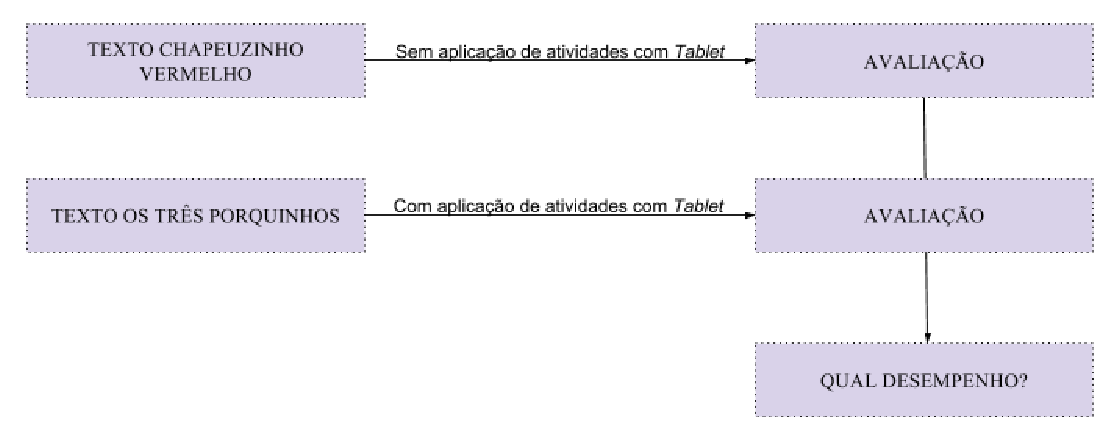
\includegraphics[scale=0.9]{metodo_de_avaliacao.eps}
\caption{Avalia��o elaborado pela pesquisadora.}
\label{fig:metodo_de_avaliacao}
\end{figure}

Avalia��o Ciclo II:

\begin{figure}[H]
\centering
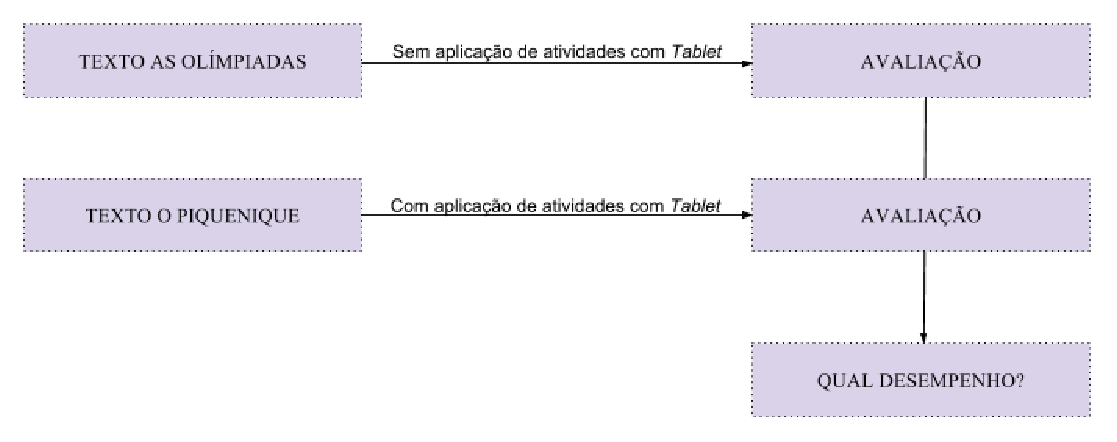
\includegraphics[scale=0.9]{metodo_de_avaliacao_2.eps}
\caption{Avalia��o elaborado pela pesquisadora.}
\label{fig:metodo_de_avaliacao_2}
\end{figure}




\chapter{Conclus\~{o}es e Perspectivas}


\section*{Perspectivas}


\subsection*{Publica\c{c}\~{o}es}



\subsection*{Submiss\~{o}es}





%=============================== Bibliografia ===============================================
\addcontentsline{toc}{chapter}{Bibliografia}
\renewcommand{\bibname}{Bibliografia}
\markboth{Bibliografia}{Bibliografia}

\bibliographystyle{dcu}
\bibliography{bibliografia}


\end{document}
